\documentclass[./RiskyContrib.tex]{subfiles}\providecommand{\econtexRoot}{}
\renewcommand{\econtexRoot}{..}

% Different execution depending on whether compiling main file or as standalone subfile
\onlyinsubfile{\externaldocument{RiskyContrib}} % Get xrefs -- esp to appendix 
%-- from main file; only works properly if main file has already been compiled; 
%order: Compile this file, then main, then this one again
\begin{document}

\hfill{\tiny \texname.tex, \today}

\begin{verbatimwrite}{RiskyContrib.title}  % Write title to .title file
A Two-Asset Savings Model with an Income-Contribution Scheme\\
REMARK
\end{verbatimwrite}

\title{A Two-Asset Savings Model with an Income-Contribution Scheme}

\author{Mateo Vel\'asquez-Giraldo}

\keywords{Lifecycle, Portfolio Choice, Social Security, Open Source}

\maketitle 

\hypertarget{abstract}{}
\begin{abstract}
This paper develops a two-asset consumption-savings model and serves as
the documentation of an open-source implementation of methods to solve and
simulate it in the \href{https://econ-ark.org/toolkit}{HARK}
toolkit \citep{carroll2018HARK}. The model represents an agent who can
save using two different assets---one risky and the other risk-free---to insure
against fluctuations in his income, but faces frictions to transferring funds between
assets. The flexibility of its implementation and its inclusion in the HARK
toolkit will allow users to adapt the model to realistic life-cycle calibrations, and
also to embedded it in heterogeneous-agents macroeconomic models.
\end{abstract}

% Various resources 
\hypertarget{links}{}
\begin{small}
\parbox{\textwidth}{
\begin{center}
\begin{tabbing}
\texttt{~Archive:~} \= \= \url{http://econ.jhu.edu/people/ccarroll/BufferStockTheory.zip} \kill \\  %
\texttt{~~GitHub:~} \> \> \url{https://github.com/Mv77/RiskyContrib} \\
\texttt{~~HARK:~} \> \> \url{https://github.com/econ-ark/HARK/} \\
\end{tabbing}
\end{center}
          
\href{https://mybinder.org/v2/gh/Mv77/RiskyContrib/main?filepath=Code\%2FPython\%2FRiskyContrib.ipynb}{CLICK HERE} for an interactive \href{https://en.wikipedia.org/wiki/Project\_Jupyter\#Jupyter_Notebook}{Jupyter Notebook} that uses the \href{https://econ-ark/HARK}{Econ-ARK/HARK} toolkit to produce our figures (warning: it may take several minutes to launch).  Information about citing the toolkit can be found at \href{https://econ-ark.org/acknowledging/}{Acknowleding Econ-ARK}.
} % end parbox{\textwidth}
\end{small}

\begin{authorsinfo}
\name{Contact: \href{mailto:mvelasq2@jhu.edu}{\texttt{mvelasq2@jhu.edu}}, \href{mailto:matthew.zahn@jhu.edu}{\texttt{matthew.zahn@jhu.edu}}, Department of Economics, 590 Wyman Hall, Johns Hopkins University, Baltimore, MD 21218, \url{https://t.co/uaflostQyF?amp=1}, \url{http://matthewvzahn.com}.}
\end{authorsinfo}

\thanks{All numerical results herein were produced using the \href{https://econ-ark/HARK}{Econ-ARK/HARK} toolkit; for further reference options see \href{https://econ-ark.org/acknowledging/}{Acknowleding Econ-ARK}.  Thanks to Chris Carroll and Sylvain Catherine for comments and guidance.}

\titlepagefinish

\newtheorem{defn}{Definition}
\newtheorem{theorem}{Theorem}

\hypertarget{Introduction}{}
\section{Introduction}



\hypertarget{The model}{}
\section{The model}

I now discuss the main components of the model informally, and leave its full
recursive mathematical representation for Section \ref{sec:recursive}.

\subsubsection{Time, mortality, and utility}

Time advances in discrete steps that I will index with $t$. The model can
be used in both infinite and finite-horizon versions.

Agents face an exogenous risk of death $\delta_t$ each period, which becomes certain at the 
maximum age of the finite-horizon version. There are no intentional bequests; agents
will consume all of their resources if they reach the last period, but they can leave
accidental bequests upon premature death.

In each period, agents derive utility from consumption only. Their utility function
follows a constant relative risk aversion specification. Formally, for a level of 
consumption $C$, the agent derives instant utility
\begin{equation}
	u(C) = \frac{C^{1-\rho}}{1- \rho}.
\end{equation}

\subsubsection{Income process}

Agents supply labor inelastically. Their labor earnings $Y_{i,t}$ are the product of a
permanent component $P_{i,t}$ and a transitory stochastic component $\theta_{i,t}$ as
in \cite{Carroll1997qje},  where $i$ indexes different agents. Formally,
\begin{equation*}
\begin{split}
\ln Y_{i,t} &= \ln P_{i,t} + \ln \theta_{i,t} \\
\ln P_{i,t} &= \ln P_{i,t-1} + \ln \Gamma_{i,t} + \ln \psi_{i,t}
\end{split}
\end{equation*}
where $\Gamma_{i,t}$ is a deterministic growth factor that can capture
life-cycle patterns in earnings, and
$\ln \psi_{i,t}\sim \mathcal{N}(-\sigma^2_{\psi,t}/2, \sigma_{\psi,t})$
is a multiplicative shock to permanent income\footnote{The mean of the shock is set so that $E[\psi_{i,t}] = 1$.}.

The transitory component $\theta_{i,t}$ is a mixture that models unemployment and
other temporal fluctuations in income as
\begin{equation*}
\ln\theta_{i,t} = \begin{cases}
\ln \mathcal{U}, & \text{With probability } \mho\\
\ln \tilde{\theta}_{i,t}\sim\mathcal{N}(-\sigma^2_{\theta,t}/2, \sigma_{\theta,t}), & \text{With probability } 1-\mho,
\end{cases}
\end{equation*}
with $\mho$ representing the probability of unemployment and $\mathcal{U}$ the replacement
factor of unemployment benefits.

This specification of the income process is parsimonious and flexible enough to accommodate
life-cycle patterns in income growth and volatility, transitory unemployment and exogenous
retirement. Introduced by \cite{Carroll1997qje}, this income specification is common in studies
of life-cycle wealth accumulation and portfolio choice; see e.g.,
\cite{Cagetti2003jbes,Cocco2005rfs,Fagereng2017jof}. The specification has
also been used in studies of income volatility, which have yielded calibrations of its stochastic
shocks' distributions \citep[see e.g.,][]{Carroll1992bpea,Carroll1997jme,Sabelhaus2010jme}

\subsubsection{Financial assets and frictions}\label{sec:fin_frictions}

Agents smooth their consumption by saving and have two assets
available for this purpose. The first is a risk-free liquid account with 
constant per-period return factor $R$. The second has a stochastic return
factor $\tilde{R}$ that is log-normally distributed and independent across
time. Various interpretations such as stocks, a retirement fund, or entrepreneurial
capital could be given to the risky asset. Importantly, consumption must be paid for
using funds from the risk-free account. The levels of risk-free and risky assets
owned by the agent will both be state variables, denoted with $M_{i,t}$ and $N_{i,t}$
respectively.

Portfolio rebalancing takes place by moving funds between the risk-free
and risky accounts. These flows are one of the agents' control variables
and are denoted as $D_{i,t}$, with $D_{i,t}>0$ representing a movement of
funds from the risk-free to the risky account. Withdrawals from the risky
account are subject to a constant-rate tax $\tau$ which can represent, for
instance, capital-gains realization taxes or early retirement-fund withdrawal
penalties. In sum, denoting post-rebalancing asset levels with $\tilde{\cdot}$,
\begin{equation*}
\begin{split}
\tilde{M}_{i,t} &= M_{i,t} - D_{i,t}(1 - 1_{[D_{i,t}\leq0]}\tau)\\
\tilde{N}_{i,t} &= N_{i,t} + D_{i,t}.
\end{split}
\end{equation*}

At any given period, an agent might not be able to rebalance his portfolio.
This ability is governed by an exogenous stochastic shock that is realized
at the start of the period
\begin{equation*}
\Adj_t \sim \text{Bernoulli}(p_t),
\end{equation*}
with $\Adj_t=1$ meaning that the agent can rebalance and $\NAdj_t=1$ ($\Adj_t = 0$)
forcing him to set $D_{i,t} = 0$. This friction is a parsimonious way to capture
the fact that portfolio rebalancing is costly and households do it sporadically.
Recent studies have advocated for \citep{Giglio2021aer} and used
\citep{Luetticke2021aej_macro} this kind of rebalancing friction.

To partially evade the possibility of being unable to rebalance their accounts, agents
can use an income deduction scheme. By default, labor income ($Y_{i,t}$) is deposited to
the risk-free liquid account at the start of every period. However, agents can pre-commit
to have a fraction  $\Contr_t\in[0,1]$ of their income diverted to their risky account instead.
This fraction can be tweaked by the agent whenever $\Adj_t = 1$; otherwise it stays at its
previous value, $\Contr_{t+1} = \Contr_t$.

\subsubsection{Timing}

\begin{figure}
\begin{center}
\resizebox{\linewidth}{!}{
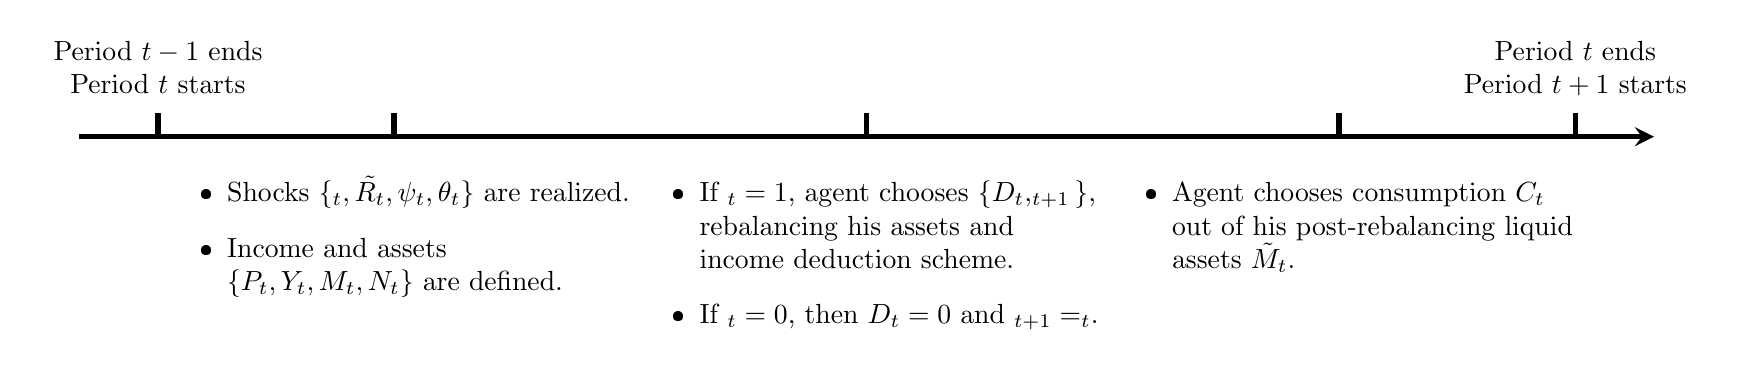
\begin{tikzpicture}
\usetikzlibrary{calc}

% draw arrow
\coordinate (start) at (-3,0);
\coordinate (end) at (17,0);

\draw [line width=2pt, -stealth] (start) -- (end);

% Priod ticks
\coordinate (period_s) at ($(start) + (1,0)$);
\coordinate (period_st) at ($(period_s) + (0,0.3)$);
\coordinate (period_e) at ($(end) - (1,0)$);
\coordinate (period_et) at ($(period_e) + (0,0.3)$);

\draw [line width=2pt] (period_s) -- (period_st);
\node [anchor=south] at (period_st.north) {\begin{tabular}{c}
Period $t-1$ ends \\ Period $t$ starts
\end{tabular}};

\draw [line width=2pt] (period_e) -- (period_et);
\node [anchor=south] at (period_et.north) {\begin{tabular}{c}
Period $t$ ends \\ Period $t+1$ starts
\end{tabular}};

% You can use `foreach` to improve the following codes
\coordinate (s0) at (1,0);
\coordinate (t0) at ($(s0)+(0,0.3)$);
\coordinate (s1) at (7,0);
\coordinate (t1) at ($(s1)+(0,0.3)$);
\coordinate (s2) at (13,0);
\coordinate (t2) at ($(s2)+(0,0.3)$);

% draw ticks
\draw [line width=2pt] (s0) -- (t0);
\node [anchor=south] at (t0.north) {};

\draw [line width=2pt] (t1) -- (s1);
\node [anchor=south] at (t1.north) {};

\draw [line width=2pt] (t2) -- (s2);
\node [anchor=south] at (t2.north) {};

% add texts
\node [anchor=north, align=left, text width=6cm] at (s0.south) {
\begin{itemize}
\item Shocks $\{\Adj_t,\tilde{R_t}, \psi_t, \theta_t\}$ are realized.
\item Income and assets $\{P_t, Y_t, M_t, N_t\}$ are defined.
\end{itemize}
};

\node [anchor=north, align=left, text width=6cm] at (s1.south) {
\begin{itemize}
\item If $\Adj_t=1$, agent chooses $\{D_t,\Contr_{t+1}\}$, rebalancing
his assets and income deduction scheme.
\item If $\Adj_t = 0$, then $D_t =0$ and $\Contr_{t+1} = \Contr_t$.
\end{itemize}
};

\node [anchor=north, align=left, text width=6cm] at (s2.south) {
\begin{itemize}
\item Agent chooses consumption $C_t$ out of his post-rebalancing
liquid assets $\tilde{M}_t$.
\end{itemize}
};
\end{tikzpicture}
}

\caption{Summary of the Model's Timing}\label{fig:Timing_diagram}
\end{center}
\end{figure}

Figure \ref{fig:Timing_diagram} summarizes the timing of stochastic shocks and
optimizing decisions that occur within a period of the life cycle model.

\hypertarget{Recursive}{}
\section{Recursive representation of the model}\label{sec:recursive}

Individual subscripts $i$ are dropped for simplicity. The value function for
an agent who is not allowed to rebalance his portfolio at time $t$ is
\begin{equation*}
    \begin{split}
V^{\NAdj}_{t}(M_t, N_t, P_t, \Contr_t) = \max_{C_t} u(C_t) 
+ p_{t+1} &\beta\delta_{t+1} E_t \left[  V^{\Adj}_{t+1}\left( M_{t+1}, N_{t+1}, 
P_{t+1} \right)\right] +\\
\left(1-p_{t+1}\right) &\beta\delta_{t+1} E_t\left[V^{\NAdj}_{t+1}\left(M_{t+1}, 
N_{t+1}, P_{t+1}, \Contr_{t+1}\right) \right]\\
\text{Subject to:} \quad &\\
0\leq& C_t \leq M_t \\
A_t =& M_t - C_t \\
M_{t+1} =& R A_t + (1-\Contr_{t+1}) Y_{t+1}\\
N_{t+1} =& \tilde{R}_{t+1}N_t + \Contr_{t+1}Y_{t+1}\\
P_{t+1} =& \Gamma_{t+1} \psi_{t+1} P_{t}\\
Y_{t+1} =& \theta_{t+1} P_{t+1}\\
\Contr_{t+1} =& \Contr_t
\end{split}
\end{equation*}
and that of agent who is allowed to rebalance is
\begin{equation*}
    \begin{split}
V^{\Adj}_{t}(M_t, N_t, P_t) = \max_{C_t,D_t,\Contr_{t+1}} 
u(C_t) + p_{t+1} &\beta\delta_{t+1} E_t \left[  V^{\Adj}_{t+1}\left( M_{t+1}, 
N_{t+1}, P_{t+1} \right)\right] +\\
\left(1-p_{t+1}\right) &\beta\delta_{t+1} E_t\left[V^{\NAdj}_{t+1}\left(M_{t+1}, 
N_{t+1}, P_{t+1}, \Contr_{t+1}\right) \right]\\
\text{Subject to:} \quad &\\
\quad -N_t \leq D_t \leq M_t, \quad \Contr_{t+1} \in& [0,1], \quad 0 \leq C_t \leq \tilde{M}_t\\
\hfill\\
\tilde{M}_t =& M_t - D_t\left(1-1_{[D_t\leq0]}\tau\right)\\
\tilde{N}_t =& N_t + D_t\\
A_t =& \tilde{M}_t - C_t \\
M_{t+1} =& R A_t + (1-\Contr_{t+1}) Y_{t+1}\\
N_{t+1} =& \tilde{R}_{t+1} \tilde{N}_t + \Contr_{t+1}Y_{t+1}\\
P_{t+1} =& \Gamma_{t+1}\psi_{t+1} P_{t}\\
Y_{t+1} =& \theta_{t+1} P_{t+1}
\end{split}
\end{equation*}

The problem can be normalized by permanent income, following
\cite{Carroll2020solvingmicrodsops}. Using lower case variables to
denote their upper-case counterparts normalized by permanent income ($x_t \equiv X_t/P_t$)
and defining $\tilde{\Gamma}_t = \Gamma_{t}\psi_{t}$, we can write
normalized problems
\begin{equation}\label{eq:bellman_NAdj_norm}
\begin{split}
v^{\NAdj}_{t}(m_t, n_t, \Contr_t) = \max_{c_t} u(c_t) 
+ p_{t+1} &\beta\delta_{t+1} E_t \left[ \tilde{\Gamma}_{t+1}^{1-\rho} v^{\Adj}_{t+1}\left( m_{t+1}, n_{t+1}\right)\right] +\\
\left(1-p_{t+1}\right) &\beta\delta_{t+1} E_t\left[\tilde{\Gamma}_{t+1}^{1-\rho} v^{\NAdj}_{t+1}\left(m_{t+1}, 
n_{t+1}, \Contr_{t+1}\right) \right]\\
\text{Subject to:} \quad &\\
0\leq& c_t \leq m_t \\
a_t =& m_t - c_t \\
m_{t+1} =& \frac{R}{\tilde{\Gamma}_{t+1}} a_t + (1-\Contr_{t+1}) \theta_{t+1}\\
n_{t+1} =& \frac{\tilde{R}_{t+1}}{\tilde{\Gamma}_{t+1}}n_t + \Contr_{t+1}\theta_{t+1}\\
\Contr_{t+1} =& \Contr_t
\end{split}
\end{equation}
and
\begin{equation}\label{eq:bellman_Adj_norm}
\begin{split}
v^{\Adj}_{t}(m_t, n_t) = \max_{c_t,d_t,\Contr_{t+1}} 
u(c_t) + p_{t+1} &\beta\delta_{t+1} E_t \left[ \tilde{\Gamma}_{t+1}^{1-\rho}  v^{\Adj}_{t+1}\left( m_{t+1}, 
n_{t+1} \right)\right] +\\
\left(1-p_{t+1}\right) &\beta\delta_{t+1} E_t\left[\tilde{\Gamma}_{t+1}^{1-\rho} v^{\NAdj}_{t+1}\left(m_{t+1}, 
n_{t+1}, \Contr_{t+1}\right) \right]\\
\text{Subject to:} \quad &\\
-n_t \leq d_t \leq m_t, \quad \Contr_{t+1} \in& [0,1], \quad 0 \leq c_t \leq \tilde{m}_t\\
\hfill\\
\tilde{m}_{t} =& m_t - d_t\left(1-1_{[d_t\leq0]}\tau\right)\\
\tilde{n}_{t} =& n_t + d_t\\
a_t =& \tilde{m}_t - c_t \\
m_{t+1} =& \frac{R}{\tilde{\Gamma}_{t+1}} a_t + (1-\Contr_{t+1})\theta_{t+1}\\
n_{t+1} =& \frac{\tilde{R}_{t+1}}{\tilde{\Gamma}_{t+1}}\tilde{n}_{t} + \Contr_{t+1}\theta_{t+1}
\end{split}
\end{equation}
It can be shown that
\begin{equation*}
V_{t}^{\Adj}(M_t,N_t,P_t) = P_t^{1-\rho} v_{t}^{\Adj}(m_t,n_t), \quad
V_{t}^{\NAdj}(M_t,N_t,P_t,\Contr_t) = P_t^{1-\rho} v_{t}^{\NAdj}(m_t,n_t,\Contr_t),
\end{equation*}
and that the policy functions of both problems are related through
\begin{equation*}
\begin{split}
C_t^{\NAdj}(M_t,N_t,P_t,\Contr_t) = P_t c_t^{\NAdj}(m_t,n_t,\Contr_t),& \quad C_t^{\Adj}(M_t,N_t,P_t) = P_t c_t^{\Adj}(m_t,n_t),\\
D_t(M_t,N_t,P_t) = P_t d_t(m_t,n_t),& \quad \Contr_{t+1}(M_t,N_t) = \Contr_{t+1}(m_t,n_t).
\end{split}
\end{equation*}
Therefore, the model's implementation solves the problem in normalized form, and re-scales
the relevant states and choices using permanent income when simulating.

\subsection{Partition into stages}

An additional insight that facilitates solving the model is that the three decisions
that an agent might take in a period (rebalancing his assets, choosing his income
deduction fraction and consuming) can be seen as happening sequentially. This is
convenient because:
\begin{itemize}
\item The sub-problems are easier to solve than the multi-choice full problem.
\item Since the non-adjusting agent only chooses his consumption and we must
solve his problem for every combination of $(m_t, n_t, \zeta_t=\zeta_{t+1})$, we can re-utilize
his solution by expressing the adjusting agent's  problem as
\begin{equation*}
v_t^{\Adj}(m_t,n_t) = \max_{\tilde{m}_t, \tilde{n}_t, \Contr_{t+1}} v_t^{\NAdj}(\tilde{m}_t, \tilde{n}_t, \Contr_{t+1}).
\end{equation*}
This insight is similar to the ``nested'' reformulation suggested by \cite{Druedahl2020compecon}.
\end{itemize}

To start re-expressing the problem, I take the order of the ageent's decisions to be:
rebalance assets, define income contribution share and finally consume. I denote the stages
at which these decisions are taken with $\Reb$, $\Sha$, and $\Cns$ respectively. I will use
$v^{\Reb}(\cdot)$, $v^{\Sha}(\cdot)$ and $v^{\Cns}(\cdot)$ to represent
\emph{stage value functions}.

I now present each stage in detail, working backwards in time.

\subsubsection{Consumption stage, $\Cns$}

An agent who takes his assets and income contribution share as given is one who
can not adjust them and can only choose his consumption. This corresponds to the
problem of the non-adjusting agent (Equation \ref{eq:bellman_NAdj_norm}). The
important facts to realize at this stage are that
\begin{equation*}
v_t^{\Adj}(m_t, n_t) = v_t^{\Reb}(m_t, n_t), \quad v_t^{\NAdj}(m_t, n_t, \Contr_t) = v_t^{\Cns}(m_t, n_t, \Contr_t),
\end{equation*}
with the first fact being true because we have assumed that asset rebalancing
is the first decision that an adjusting agent takes, and he assumes that his
subsequent decisions will be optimal. Therefore, the consumption stage problem is
\begin{equation}\label{eq:bellman_cns}
\begin{split}
v^{\Cns}_{t}(\tilde{m}_t, \tilde{n}_t, \Contr_{t+1}) = \max_{c_t} u(c_t) 
+ p_{t+1} &\beta\delta_{t+1} E_t \left[ \tilde{\Gamma}_{t+1}^{1-\rho} v^{\Reb}_{t+1}\left( m_{t+1}, n_{t+1}\right)\right] +\\
\left(1-p_{t+1}\right) &\beta\delta_{t+1} E_t\left[\tilde{\Gamma}_{t+1}^{1-\rho} v^{\Cns}_{t+1}\left(m_{t+1}, 
n_{t+1}, \Contr_{t+1}\right) \right]\\
\text{Subject to:} \quad &\\
0\leq& c_t \leq \tilde{m}_t \\
a_t =& \tilde{m}_t - c_t \\
m_{t+1} =& \frac{R}{\tilde{\Gamma}_{t+1}} a_t + (1-\Contr_{t+1}) \theta_{t+1}\\
n_{t+1} =& \frac{\tilde{R}_{t+1}}{\tilde{\Gamma}_{t+1}}\tilde{n}_t + \Contr_{t+1}\theta_{t+1}
\end{split}
\end{equation}

\subsubsection{Income contribution share stage, $\Sha$}

An agent with the option to set his income contribution share will do so
taking his asset allocation as given and assuming that he will optimally
pick his consumption in the next stage. His problem is
\begin{equation}\label{eq:bellman_sha}
v_t^{\Sha}(\tilde{m}_t,\tilde{n}_t) = \max_{\zeta_{t+1}\in[0,1]} v^{\Cns}_{t}(\tilde{m}_t, \tilde{n}_t, \Contr_{t+1})
\end{equation}

\subsubsection{Rebalancing stage, $\Reb$}

The first decision that an agent takes, if allowed, is how to reallocate his
assets. At this stage, his value function is
\begin{equation}\label{eq:bellman_reb}
\begin{split}
v^{\Reb}_{t}(m_t, n_t) =& \max_{d_t} v_t^{\Sha}(\tilde{m}_t, \tilde{n}_t)\\
\text{Subject to:} \quad &\\
-n_t \leq& d_t \leq m_t\\
\tilde{m}_{t} =& m_t - d_t\left(1-1_{[d_t\leq0]}\tau\right)\\
\tilde{n}_{t} =& n_t + d_t\\
\end{split}
\end{equation}

The solution to this stage problem will be the policy function $d_t(\cdot, \cdot)$
that gives the optimal flow from risk-free to risky assets, which can be negative.
However, it is convenient to define a normalized policy function $\dFrac_t$ as
\begin{equation*}
\dFrac_t(m, n) = \begin{cases}
d_t(m,n)/m, & \text{ if } d_t(m,n) \geq 0 \\
d_t(m,n)/n, & \text{ if } d_t(m,n) < 0
\end{cases}
\end{equation*}
so that $-1 \leq \dFrac(m,n) \leq 1$ for all $(m,n)$.

\hypertarget{Examples}{}
\section{Examples of Solutions and Simulations}

This section examines various instances of the model under
different specifications for lives' lengths and financial
frictions. The main purpose of these exercises is to illustrate
the model's capabilities and the implications of financial
frictions for asset allocations.

\subsection{Infinite-horizon}

For a first exercise, consider the infinite-horizon version of
the model. In this version, parameters are constant and the
optimization problem that the agent solves every period
is---up to the values of state variables---the same. I set
the parameters to the values reported in Table \ref{tab:inf_calibration}.

\begin{table}
\begin{center}
\caption{Infinite Horizon Example Calibration}\label{tab:inf_calibration}
\begin{tabular}{ccc}
\toprule
Name in HARK & Mathematical Symbol & Value \\
\midrule
\texttt{CRRA} & $\rho$ & $5.0$ \\
\texttt{Rfree} & $R$& $1.03$ \\
\texttt{DiscFac} & $\beta$ & $0.9$ \\
\texttt{LivPrb} & $\delta$ &  $0.98$ \\
\texttt{PermGroFac} & $\Gamma$ &  $1.01$ \\
\texttt{PermShkStd} & $\sigma_\psi$ &  $0.1$ \\
\texttt{TranShkStd} & $\sigma_\theta$ &  $0.1$ \\
\texttt{UnempPrb} & $\mho$ &  $0.05$ \\
\texttt{IncUnemp} & $\mathcal{U}$ &  $0.3$ \\
\texttt{RiskyAvg} & $E[\tilde{R}]$ &  $1.08$ \\
\texttt{RiskyStd} & $\sqrt{V[\tilde{R}]}$ &  $0.18$ \\
\texttt{AdjustPrb} & $p$ &  Varying \\
\texttt{tau} & $\tau$ & Varying \\
\bottomrule
\end{tabular}
\end{center}
\end{table}

The infinite-horizon solution is obtained by value-function iteration
backwards in time. I define trivial starting value functions $v^{\Adj}_T(\cdot)$
and $v^{\NAdj}_T(\cdot)$ and use Equations \ref{eq:bellman_Adj_norm} and
\ref{eq:bellman_NAdj_norm} to find $v^{\Adj}_{T-1}(\cdot)$ and $v^{\NAdj}_{T-1}(\cdot)$.
I repeat this process until the value functions obtained in successive
iterations are similar enough.

To illustrate the effect of the different financial frictions in the
model, I present solutions for three different parametrizations.
\begin{itemize}
\item \textbf{Base}: a version without financial frictions. The probability
of being able to rebalance is $p = 1$ and the risky withdrawal tax rate is $\tau = 0$.
\item \textbf{Tax}: a version with a risky withdrawal tax of $10\%$ ($\tau = 0.1$).
The probability of being able to rebalance is $p = 1$.
\item \textbf{Calvo}: a version with a stochastic inability to rebalance that
occurs with a $75\%$ chance ($p = 0.25$). The risky withdrawal is $\tau = 0$.
\end{itemize}

\hypertarget{inf_dFunc}{}
\begin{figure}[tbp]
\centerline{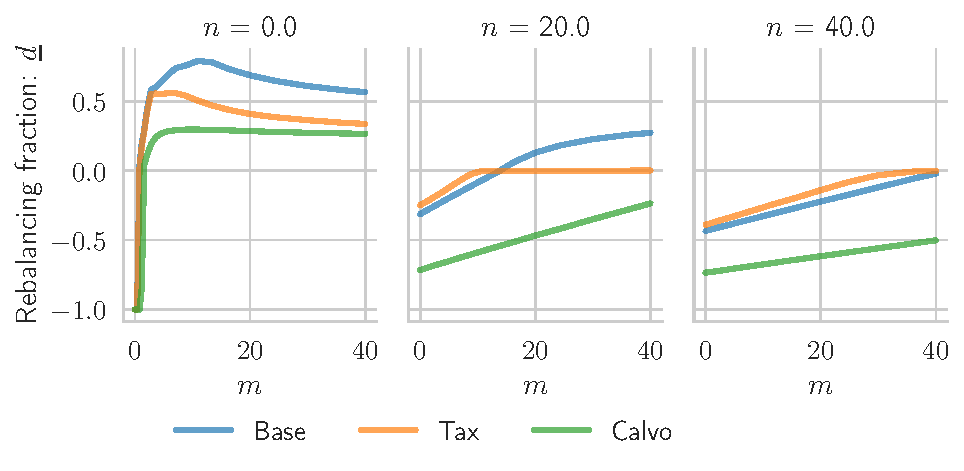
\includegraphics[]{\FigDir/inf_dFunc}}
\caption{Optimal rebalancing fraction $\dFrac$ in the infinite horizon model.}
\label{fig:inf_dFunc}
\end{figure}

The first stage of an agent's period (if he is allowed to rebalance) is to
solve the asset-rebalancing problem (Equation \ref{eq:bellman_reb}). The solution
to this problem is the rebalancing fraction function $\dFrac(m,n)$, which I present
in Figure \ref{fig:inf_dFunc} for the different parametrizations and various
combinations of $(m,n)$. The figure shows how individuals with low risk-free resources
withdraw funds from their risky accounts in order to finance their consumption.
The version of the model with the withdrawal tax has regions where $\dFrac = 0$ as
a result of the tax's asymmetry---these are regions where the marginal utility of the
risk-free asset lies between the pre-tax and post-tax marginal utility of risky assets.
Finally, as illustrated by the figure, the stochastic inability to rebalance pushes agents to
keep less funds in the risky asset, withdrawing them at higher rates when they get the chance.

\hypertarget{inf_ShareFunc}{}
\begin{figure}[tbp]
\centerline{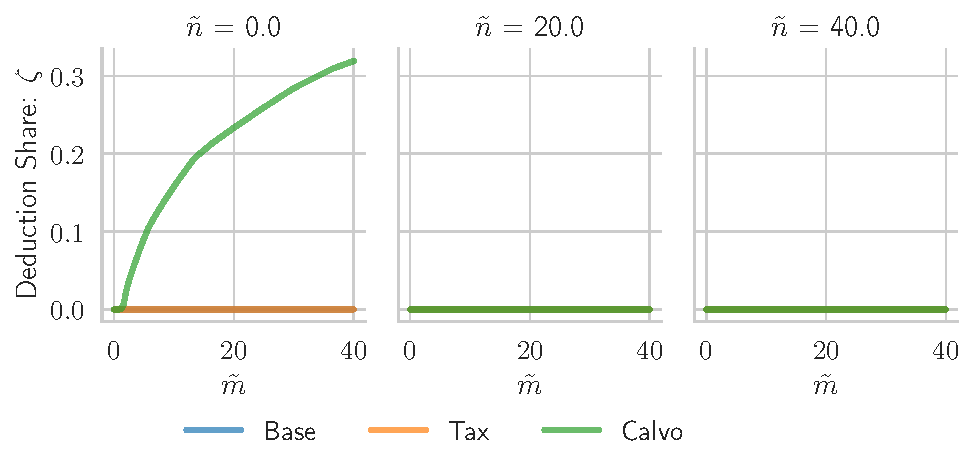
\includegraphics[]{\FigDir/inf_ShareFunc}}
\caption{Optimal income contribution share $\Contr$ in the infinite horizon model.}
\label{fig:inf_ShareFunc}
\end{figure}

The second stage in a period, which an agent also participates in only if
he draws $\Adj_t = 1$, consists of choosing the income contribution share $\Contr$.
Figure \ref{fig:inf_ShareFunc} presents the policy function $\Contr(\tilde{m},\tilde{n})$
for various $(\tilde{m},\tilde{n})$ combinations. The income deduction scheme
becomes irrelevant in the ``Base'' and ``Tax'' versions of the model, since
agents are always able to rebalance their assets ($p=1$) and thus pre-committing
funds has o benefits. The figure shows that when $p<1$ agents will
make use of the system, especially if the agent has low risky asset balances.

\hypertarget{inf_cFunc}{}
\begin{figure}[tbp]
\centerline{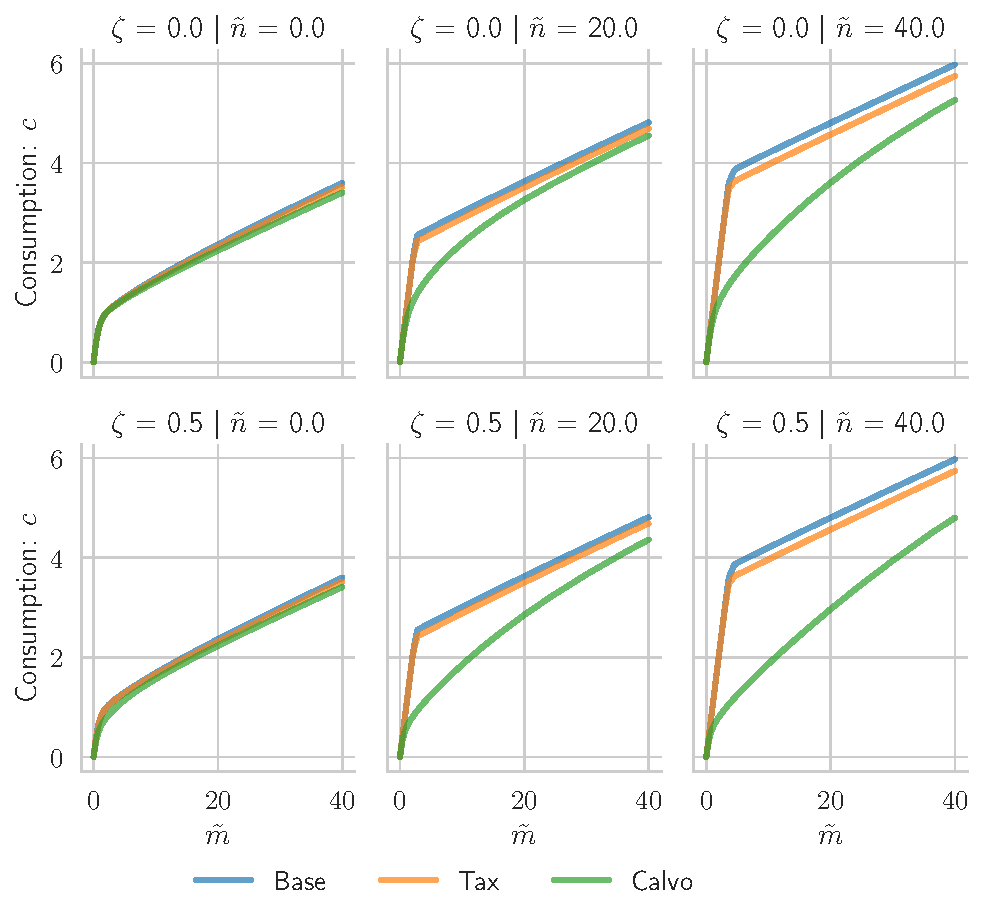
\includegraphics[]{\FigDir/inf_cFunc}}
\caption{Convergence of the Consumption Rules}
\label{fig:inf_cFunc}
\end{figure}

The final stage in the agent's problem, or the only one if $\Adj_t=0$, is
to choose how much of his risk-free resources to consume. Figure \ref{fig:inf_cFunc}
presents the consumption functions for different combinations of post-rebalancing
assets $(\tilde{m}, \tilde{n})$ and income contribution fractions $\Contr$. Consumption
is increasing in both assets and financial frictions reduce the
level of consumption at any given state. A first characteristic to note is that
the contribution share has no effect on the consumption functions of the ``Base'' model
and little effect in those of the ``Tax'' model. Since these agents know they will be
able to rebalance their assets, the only relevance of where their income is initially
deposited comes from potentially paying the rebalancing tax. A second notable aspect is
the interaction of financial frictions and saving choices. The figure shows that each
of the frictions produces leftward shifts in the points at which the consumer switches
from consuming all of his liquid resources ($c = \tilde{m}$) to saving ($c < \tilde{m}$).


\hypertarget{inf_rebalance_Base}{}
\begin{figure}[tbp]
\centerline{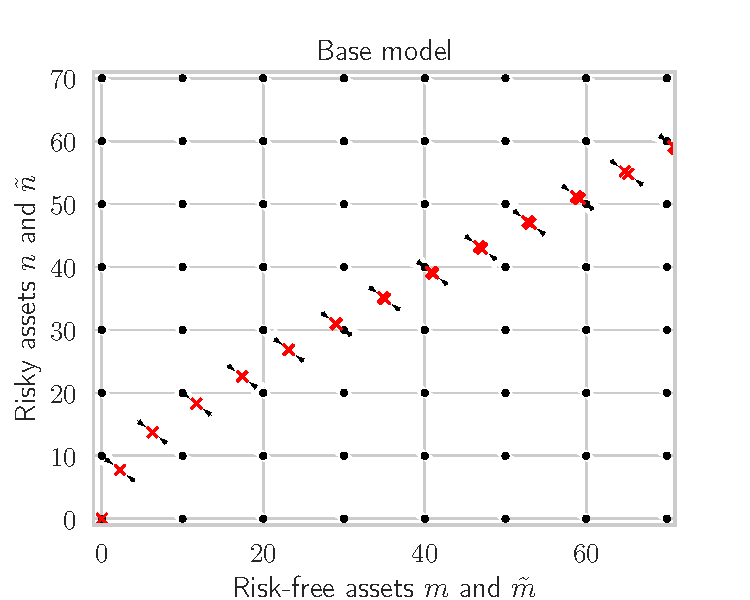
\includegraphics[]{\FigDir/inf_rebalance_Base}}
\caption{Convergence of the Consumption Rules}
\label{fig:inf_dFunc}
\end{figure}
\hypertarget{inf_rebalance_Tax}{}
\begin{figure}[tbp]
\centerline{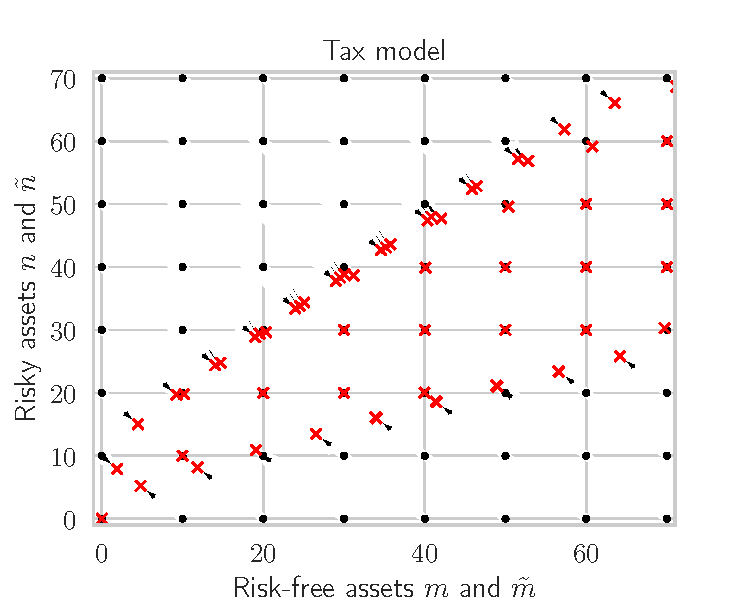
\includegraphics[]{\FigDir/inf_rebalance_Tax}}
\caption{Asset rebalancing in the ``Calvo'' model.}
\label{fig:inf_rebalance_Tax}
\end{figure}
\hypertarget{inf_rebalance_Calvo}{}
\begin{figure}[tbp]
\centerline{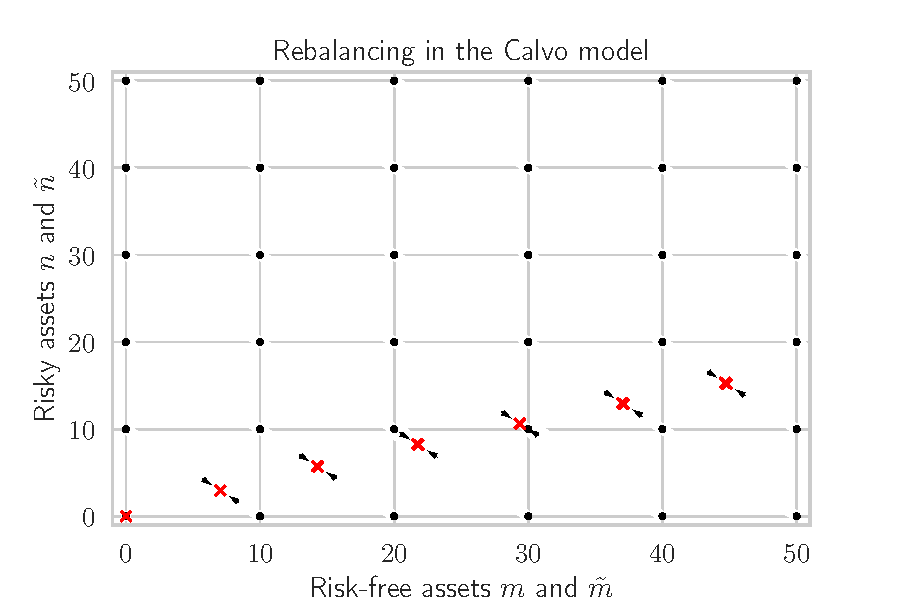
\includegraphics[]{\FigDir/inf_rebalance_Calvo}}
\caption{Asset rebalancing in the model with a withdrawal tax.}
\label{fig:inf_rebalance_Calvo}
\end{figure}

Figures \ref{fig:inf_rebalance_Base}, \ref{fig:inf_rebalance_Tax} and
\ref{fig:inf_rebalance_Calvo} give a visual representation of the agents'
reallocation decisions and the effect that financial frictions have on them.
For various starting asset allocations $(m,n)$ represented with black dots,
each of the plots displays the optimal post-rebalancing allocation
$(\tilde{m},\tilde{n})$  with a red cross, joining initial and final positions
with arrows. Figure \ref{fig:inf_rebalance_Base} shows that in the frictionless
``Base'' model every initial point in a $m+n=x$ line maps to the same post-rebalancing
portfolio, and that these portfolios lean towards risk-free assets as total wealth
increases (they start above the $45$-degree line but move below it as $m+n$ increases).
Figure \ref{fig:inf_rebalance_Tax} introduces the rebalancing tax, which creates
a region in which the agent does not rebalance his portfolio. This zone of
inaction is a different representation of the flat regions of the $\dFrac(\cdot)$
function in Figure \ref{fig:inf_dFunc}. The tax also rotates the south-east pointing
arrows, as a unit of $n$ now transforms into less than a unit of $m$. Finally,
Figure \ref{fig:inf_rebalance_Calvo} removes the tax and introduces the stochastic
inability to rebalance, which closes the inaction zone but makes the risky asset
less desirable, resulting in an optimal portfolio trajectory that is closer to
the horizontal axis.


\subsection{Life-Cycle finite horizon}

The finite-horizon version of the model represents agents that live for up to
a maximum finite number of periods and might face different parametrizations
of their problem (taxes, income patterns, etc) in each period. This version is
well-suited for representing microeconomic life-cycle problems of savings and
portfolio decisions, and for using its agents in overlapping-generations macroeconomic
models. This section presents life-cycle simulations of the model under different
parametrizations for financial frictions, showing the effect that they produce
on wealth accumulation and portfolio choice.

I maintain the preferences ($\rho$, $\beta$) and financial-asset properties
($R$, $E[\tilde{R}]$, $V[\tilde{R}]$) from Table \ref{tab:inf_calibration}.
Survival probabilities $\delta$, and income's growth factor and volatilities
($\Gamma$, $\sigma_{\psi}$, $\sigma_{\theta}$) are now time-varying and
calibrated to represent  individuals who enter the model at age 25,
retire exogenously at 65, and live to a maximum age of 90. Survival
probabilities come from the 2004 SSA life-tables for males. Income growth
factors and volatilities come from the calibration for high-school graduates
in \cite{Cagetti2003jbes}. The parametrizations of the model differ in their
assumptions about financial frictions. I present the following four configurations:
\begin{itemize}
\item \textbf{Base}: the probability of being able to rebalance is $p = 1$
and the risky withdrawal tax rate is $\tau = 0$, both constant throughout the agents' lives.
\item \textbf{Tax}: the risky withdrawal tax is constant at $10\%$ and the agents
can always rebalance their portfolios.
\item \textbf{Calvo}: there is no risky withdrawal tax, but there is only a $25\%$ chance
that agents can rebalance their portfolios every year.
\item \textbf{Retirement}: there is no risky withdrawal tax, but the agents' ability
to rebalance their portfolio is time-varying; they can rebalance their assets and pick
their income-deduction scheme for certain when they enter the model at age 25, but
then they have no chance of doing so again ($p=0$) until they retire. After retirement
at age 65, they can always rebalance their portfolio ($p=1$).
\end{itemize}

\hypertarget{LC_age_profiles}{}
\begin{figure}[tbp]
\centerline{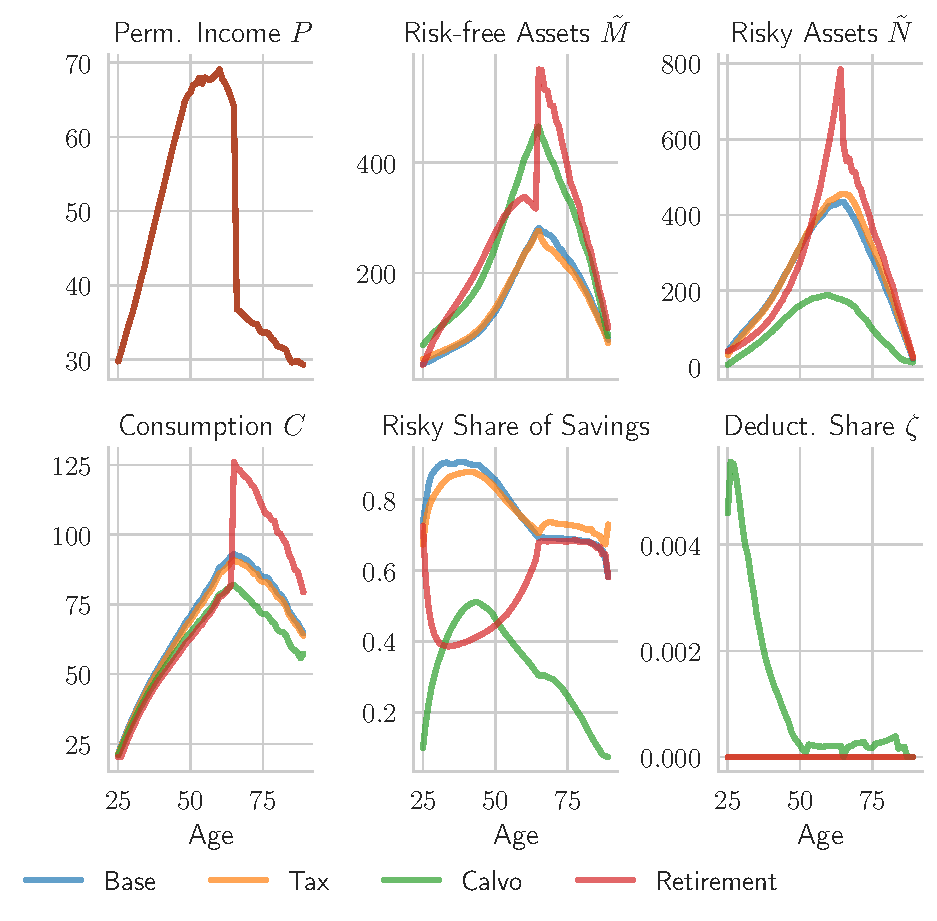
\includegraphics[]{\FigDir/LC_age_profiles}}
\caption{Age profiles of variables of interest in life-cycle calibrations}
\label{fig:LC_age_profiles}
\end{figure}


I simulate populations of $50$ agents for $5,000$ periods with each of the
parametrizations. Each time an agent dies, he is replaced by a new 25-year-old.
I calculate age profiles of various variables of interest by finding their
averages across all the simulated observations of every given age. Figure 
\ref{fig:LC_age_profiles} presents the age profiles of permanent income,
asset balances, the risky share of savings, and the income deduction share
for all parametrizations.

The age profiles of the ``Base'' and ``Tax'' parametrizations are similar.
The risky share of savings, which I define as $\tilde{N}/(A + \tilde{M})$,
follows the same pattern as in \cite{Cocco2005rfs}, starting high and declining
with age. The main difference between both calibrations is that the tax
makes agents' risky share lower when they are young (because of an unwillingness
to pay the tax if they are forced to draw from their scarce wealth) and higher
after retirement as the tax incentivizes them to withdraw their funds more slowly.
Since in both calibrations the agent can rebalance his portfolio each period, there
is no reason to use the income deduction scheme.

Matters change substantially with the stochastic inability to rebalance. As Figure
\ref{fig:LC_age_profiles} shows, agents under the ``Calvo'' calibration accumulate
less risky asset balances. In part, this is due to the mechanical effect of a reduced
chance of being able to shift funds into the risky asset. However, risky assets also
become less desirable at young ages since they are worse at insuring agents against
their income fluctuations---they might be barred from accessing their funds precisely
at a period when they fall unemployed. The uncertain ability to extract funds from the
risky asset also reduces its appeal as a vehicle for retirement savings, which is
evidenced in a low income deduction share. As a result of investing less in the risky
asset, agents in this calibration accumulate less total wealth and can afford only a
lower level of consumption.

The last calibration, ``Retirement'', shows what happens when the rebalancing friction
negates the risky asset's use as a buffer for income fluctuations at younger ages but
maintains its attractiveness as a vehicle for retirement savings. In this calibration,
agents use the income-deduction scheme to progressively build up their stock of risky
assets. The average contribution share is high enough that these agents accumulate the
most risky assets by retirement out of all calibrations. When they retire, as they can
finally access their risky funds, they afford a higher level of consumption than the
other types of agent.

These exercises show how the different financial frictions that the model can
accommodate generate different consumption, savings, and portfolio patterns.


\hypertarget{Conclusion}{}
\section{Conclusion}

\hypertarget{Puzzles-and-Questions}{}
\section{Puzzles and Questions}\label{sec:Puzzles}

\hypertarget{Robustness Analyses}{}
\section{Robustness Analyses}

\clearpage\vfill\eject

\onlyinsubfile{\bibliography{\econtexRoot/RiskyContrib-Add}}

\end{document}
